% !TeX root = ../main.tex
\documentclass[./../main.tex]{subfiles}

\begin{document}
\section{Triển khai}
Phần mềm được phát triển bằng công cụ hỗ trợ lập trình Visual Studio Code (\acrshort{vsc}), được phát triển bởi Microsoft và Electron Framework, cho các hệ điều hành như Windows, Linux và macOS. Công cụ này bao gồm các tính năng giúp cho việc gỡ lỗi, gợi ý câu lệnh, định dạng lại mã lệnh theo các quy chuẩn, quản lý mã nguồn với Github và các tiện ích mở rộng khác. Để cho việc phát triển phần mềm và gỡ lỗi khi cần được diễn ra nhanh chóng, trong quá trình triển khai sẽ chạy trực tiếp trên localhost để thấy được sự thay đổi gần như là ngay lập tức khi sửa mã nguồn. Nhờ sử dụng Github để quản lý mã lệnh mà việc triển khai phần mềm có thể diễn ra ở mọi nơi, và có thể kiểm thử trên nhiều hệ điều hành như Windows, Linux.

Từ phân tích và thiết kế của các phần trước, việc phát triển phần mềm diễn ra khá thuận tiện. Tuy nhiên khi gặp một số vấn đề hay nhận thấy các phân tích hoặc thiết kế không phù hợp, bị thiếu sót, thì có thể sửa đổi lại để đảm bảo sản phẩm có mức độ hoàn thiện tốt hơn. Ví dụ như tính tương thích về giao diện của trang web chưa phù hợp với thiết bị điện thoại thông minh, thì cần khắc phục bằng cách cấu hình lại bố cục giao diện tùy theo thiết bị mà người dùng sử dụng, từ đó tính hoàn thiện của sản phẩm sẽ tốt hơn, đáp ứng được nhiều hơn nhu cầu của người dùng.

Những công cụ được sử dụng trong phần triển khai bao gồm:
\begin{itemize}
    \item Visual Studio Code: Viết mã nguồn, định dạng lại các tệp dữ liệu và mã lệnh, hỗ trợ thực thi phần mềm và gỡ lỗi.
    \item Docker: Chạy phần mềm trên máy cá nhân trước khi phát hành phiên bản mới lên máy chủ.
    \item Các phần mềm, tiện ích xem và sửa tệp csv: Vì dữ liệu trong cơ sở dữ liệu có thể được nhập, xuất bằng tệp dữ liệu dạng csv nên nhờ các công cụ này có thể xem và sửa các tệp đó một cách trực quan.
    \item Github: Quản lý mã nguồn và hỗ trợ cho việc triển khai từ nhiều thiết bị khác nhau được đồng bộ.
    \item Github Copilot: Một công cụ \acrshort{ai} cung cấp cho nhà phát triển các đề xuất khi viết mã lệnh dựa trên ngôn ngữ, các hàm, dữ liệu tương quan, các nhận xét, và trong ngữ cảnh của phần đang được chỉnh sửa nhờ sự đóng góp của cộng đồng và có thể tự động cá nhân hóa.
    \item Windows Subsystem for Linux: Hỗ trợ việc chạy hệ điều hành Linux cho các máy tính Windows, trong dự án này thì được sử dụng để chạy Docker cho phía backend và frontend trên máy Windows.
\end{itemize}

\section{Cài đặt}
Khi phần phát triển dự án đã tương đối hoàn thiện, phần mềm sẽ có thể bắt đầu công đoạn cài đặt. Sử dụng Google Cloud Platforms(\acrshort{gcp}), một nền tảng điện toán đám mây, và Docker, Docker compose, phần mềm theo dõi sắn KOICA đã được cài đặt trên máy chủ phi vật lý phục vụ cho mục đích kiểm thử và phát hành sản phẩm.

\subsection{Google Cloud Platforms}
Chuyển đổi kỹ thuật số từ việc chạy máy chủ vật lý tại cơ sở hạ tầng cũ sang điện toán đám mây có thể giúp tiết kiệm chi phí và thuận tiện hơn cho việc quản lý mọi lúc, mọi nơi và bởi những người có thẩm quyền. Google Cloud là nền tảng điện toán đám mây do Google phát triển và được phát hành lần đầu vào tháng 4 năm 2008, đây là nền tảng bao gồm một loạt các dịch vụ có khả năng tính toán, lưu trữ và triển khai ứng dụng chạy trên phần cứng của Google, thường được sử dụng cho việc phát triển backend. \acrshort{gcp} cung cấp các dịch vụ như cơ sở hạ tầng, nền tảng cho việc phát triển môi trường máy tính không có máy chủ, là một phần của Google Cloud. Bằng các công cụ Google Cloud Console, Compute Engine gồm Virtual Machine instances và Firewall rules, Docker và Docker compose, máy chủ đã được cài đặt và chạy trên điện toán đám mây.

\subsection{Các bước cài đặt}
Để cài đặt phần mềm trên điện toán đám mây trước tiên cần tìm hiểu về các công cụ cần để sử dụng. Sau khi đã nắm được cơ bản mục đích sử dụng của từng công cụ sẽ tiến hành cài đặt theo các bước sau:

\begin{itemize}
    \item \textbf{Bước 1: Chuẩn bị, khởi tạo tài khoản và công cụ.}\\
    Để có thể sử dụng các bộ công cụ của \acrshort{gcp} , người dùng cần phải có tài khoản Google và thẻ Visa hoặc thẻ MasterCard để sử dụng cho việc thanh toán nếu cần. \acrshort{gcp} hiện đang hỗ trợ người dùng mới bằng cách miễn phí 3 tháng và hơn 7 triệu VND chi phí khi sử dụng các bộ công cụ nếu tạo và xác minh tài khoản \acrshort{gcp} thành công. Sau khi có tài khoản, tiếp tục tiến hành tạo máy ảo trong Google Compute Engine, phần \acrshort{vm} instances ở thanh công cụ bên trái màn hình. Khi tạo mới một máy ảo, cần để ý các thông tin như khu vực, vùng cài đặt, các cài đặt về máy ảo như hệ điều hành, số \acrshort{cpu} , bộ nhớ máy và cài đặt tường lửa.\\
    Phần mềm theo dõi sắn KOICA sử dụng máy ảo chạy hệ điều hành Ubuntu 20.04, một bộ xử lý ảo (\acrshort{vcpu}), 3.75GB RAM, kiến trúc máy là x86/64, tường lửa chấp nhận cho phương thức \acrshort{http} và \acrshort{https}, được cài đặt ở khu vực us-east1-b, và sử dụng địa chỉ \acrshort{ipv4}.
    \item \textbf{Bước 2: Lấy mã nguồn từ Github.}\\
    Nhờ việc quản lý mã nguồn trên Github, việc lấy mã và các phiên bản phần mềm có thể dễ dàng thực hiện trên máy chủ. Hiện nay, Github khuyến khích dùng mã \acrshort{ssh} để tạo mã và xác thực với thiết bị và tài khoản để tải mã nguồn. Sau khi cài đặt xong phần xác thực thiết bị máy ảo với Github và tài khoản tương ứng có chứa mã nguồn, tải mã phần backend và frontend lần lượt về máy ảo bằng câu lệnh sau:\\
    \begin{verbatim}
    git clone git@github.com:lmhuong711/kltn-be.git \
    git clone git@github.com:lmhuong711/kltn-fe.git
    \end{verbatim}
    \item \textbf{Bước 3: Thực thi cài đặt frontend và backend trên máy ảo.}\\
    Sau khi máy ảo đã chứa mã nguồn của phần mềm, thì cần tạo các tệp .env chứa các biến môi trường tương tự như .env.example cho cả backend và frontend. Kiểm tra lại các biến môi trường đã đúng chưa rồi mới cài đặt phần mềm. Thực hiện các câu lệnh sau trên dòng lệnh bên trong từng tập mã nguồn của backend và frontend. Khuyến khích thực thi trên backend trước.
    \begin{verbatim}
    docker-compose pull \
    docker-compose build --no-cache \
    docker-compose up --build -d
    \end{verbatim}
    Lệnh \texttt{docker-compose pull} để kéo một image được liên kết với một dịch vụ đã được chỉ định trong compose.yaml. Sau đó thực thi \texttt{docker-compose build --no-cache} để xây dựng phần mềm trên máy ảo với tham số --no-cache để đảm bảo việc xây dựng từ đầu và không bị lưu bộ nhớ đệm. Cuối cùng để phần mềm luôn khả dụng thì cần đảm bảo container sẽ phải chạy ngầm bằng lệnh \texttt{docker-compose up --build -d}.\\
    Lưu ý khi cài đặt cần đảm bảo các quyền của người dùng trong dòng lệnh, khuyến khích thực thi dưới vai trò là root. Riêng phía backend, cần chạy thêm câu lệnh sau để cho phép tải và lưu các tệp ảnh vào cơ sở dữ liệu: \texttt{docker-compose exec -u root directus chown -R node:node /directus/database \\ /directus/uploads}.
    \item \textbf{Bước 4: Cài đặt tường lửa cho hệ thống.}\\
    Khi phần mềm đã được chạy bằng Docker compose thành công, nếu như chưa cài đặt tường lửa lúc tạo máy ảo thì cần phải làm bước này để phần mềm được công khai sử dụng trên mạng Internet. Nếu đã cấu hình tường lửa cho tối thiểu một trong hai phương thức \acrshort{http} hoặc \acrshort{https} thì có thể bỏ qua bước này. Nếu chưa thì cần chọn phương thức phù hợp cho tường lửa hoặc tự tạo thẻ tag cấu hình phù hợp với mục đích sử dụng và gắn với hệ thống.
    \item \textbf{Bước 5: Kiểm tra và xác nhận cài đặt.}\\
    Hoàn thành đủ các bước trên là công việc cài đặt phần mềm thành công. Cần vào đường dẫn tương ứng với backend và frontend để kiểm tra và xác nhận xem phần mềm đã chạy đúng như mong đợi chưa, tiến hành sửa lỗi nếu cần.
\end{itemize}

\section{Kiểm thử}
Phần này sẽ ghi lại tổng kết của việc kiểm thử bằng các kịch bản kiểm thử, quan sát kết quả, và đánh giá chức năng có hoạt động đúng như mong đợi. Pha kiểm thử được thực hiện xuyên suốt quá trình phát triển phần mềm, sử dụng trực tiếp giao diện trang web để kiểm thử \acrshort{api} lẫn giao diện và được kiểm tra trên các trình duyệt khác nhau cũng như các hệ điều hành khác nhau:
\begin{itemize}
    \item Google Chrome phiên bản 112.0.5615.138 (Phiên bản Chính thức) (64 bit) trên Windows 10 và phiên bản 112.0.5615.165-1 trên Ubuntu 20.04.
    \item Microsoft Edge phiên bản 112.0.1722.48 (Phiên bản Chính thức) (64 bit) trên Windows 10. 
    \item Firefox phiên bản 112.0.1 (Phiên bản Chính thức) (64 bit) trên Window 10.  
\end{itemize}

\subsection{Kiểm thử yêu cầu chức năng}
\subsubsection{Kế hoạch kiểm thử}
Dưới đây là các chức năng đã được kiểm thử:
\begin{longtable}{| p{0.07\linewidth} | p{0.25\linewidth} | p{0.58\linewidth} |}
\caption{Danh sách các ca kiểm thử thủ công} \label{test-case-list}
\hline
\textbf{STT} & \textbf{Nhóm chức năng} & \textbf{Các ca kiểm thử} \\ \hline 
    \centerline{1} & 
    Quản lý tài khoản & 
    - Đăng ký tài khoản \newline
    - Đăng nhập \newline
    - Sửa thông tin tài khoản \newline
    - Đăng xuất \newline
    - Tạo nhận xét
\\ \hline
    \centerline{2} & 
    Tổng hợp thông tin về sắn, bệnh trên cây sắn &
    - Hiển thị danh sách \newline
    - Tìm kiếm thông tin sắn, bệnh trên cây sắn \newline
    - Lọc danh sách \newline
    - Xem chi tiết thông tin sắn, bệnh trên cây sắn  \newline 
    - Phân trang \newline 
    - Sắp xếp danh sách \newline
    - Làm mới danh sách
\\ \hline
    \centerline{3} & 
    Bản đồ sắn & 
    - Hiển thị bản đồ cùng các điểm đánh dấu \newline
    - Lọc dịch bệnh \newline
    - Xem chi tiết dịch bệnh tại điểm đánh dấu \newline 
    - Làm mới danh sách dịch bệnh \newline 
    - Điều hướng đến các liên kết khác
\\ \hline
    \centerline{4} & 
    Chẩn đoán bệnh bằng hình ảnh &
    - Tải ảnh lên \newline
    - Hiển thị thông tin các bệnh được chuẩn đoán 
\\ \hline
    \centerline{5} & 
    Danh sách nguồn cung sắn &
    - Hiển thị danh sách nguồn cung \newline
    - Lọc danh sách nguồn cung \newline
    - Sắp xếp danh sách nguồn cung \newline
    - Làm mới danh sách nguồn cung \newline
    - Phân trang 
\\ \hline
    \centerline{6} & 
    Thương mại sắn &
    - Hiển thị danh sách đề xuất \newline
    - Lọc danh sách đề xuất \newline
    - Sắp xếp danh sách đề xuất \newline
    - Làm mới danh sách đề xuất \newline
    - Tạo đề xuất \newline
    - Sửa đề xuất \newline
    - Xóa đề xuất \newline
    - Phân trang  
\\ \hline
    \centerline{7} & 
    Diễn đàn &
    - Hiển thị danh sách bài viết \newline
    - Lọc bài viết \newline
    - Tìm bài viết \newline
    - Làm mới danh sách bài viết \newline
    - Tạo bài viết \newline
    - Phân trang  
\\ \hline
    \centerline{8} & 
    Quản lý phần mềm đối với quản trị viên &
    - Hiển thị dữ liệu \newline
    - Thêm dữ liệu \newline
    - Sửa dữ liệu \newline
    - Xóa dữ liệu \newline
    - Xác minh tài khoản \newline
    - Tạo người dùng hoặc quản trị viên
\\ \hline
\end{longtable}

\subsubsection{Kịch bản kiểm thử}
Các chức năng bên trên được tiến hành kiểm thử từ tháng 03/2023. Như đã đề cập ở trên, quá trình kiểm thử được diễn ra một cách thủ công qua các kịch bản được xây dựng sẵn. Mỗi ca kiểm thử đều sử dụng nhiều kịch bản khác nhau cho cả kiểm thử tích cực (positive testing) và kiểm thử tiêu cực (negative testing), hầu hết kết quả của các ca kiểm thử đều đúng như kì vọng của kịch bản. Những ca kiểm thử chưa đạt yêu cầu thì cần tiến hành tìm nguyên nhân và chữa lỗi, các lỗi không gây ảnh hưởng nghiêm trọng đến việc vận hành phần mềm nhưng cũng cần sửa đổi để trải nghiệm người dùng không bị ảnh hưởng. Dưới đây là một số kịch bản đã được dùng để kiểm thử:
\clearpage

\begin{longtable}{| p{0.07\linewidth} | p{0.35\linewidth} | p{0.35\linewidth} | p{0.12\linewidth} |}
\caption{Kiểm thử đăng ký} \label{test-case-1}
\hline
\textbf{STT} & \textbf{Kịch bản kiểm thử} & \textbf{Kì vọng} & \textbf{Kết quả}
\\ \hline 
    \centerline{1} & 
    - Tên kịch bản: Nhập thiếu thông tin biểu mẫu\newline 
    - Dữ liệu kiểm thử: Nhập đúng các trường thông tin trừ trường số điện thoại &
    Trường số điện thoại có viền đỏ, bên dưới có thông báo 'Vui lòng nhập số điện thoại!' &
    \centerline{Đạt}
\\ \hline 
    \centerline{2} & 
    - Tên kịch bản: Nhập sai định dạng email\newline
    - Dữ liệu kiểm thử: Email: \textbf{mail.com}, các trường còn lại nhập đúng &
    Trường email có viền đỏ, bên dưới có thông báo 'Email không hợp lệ!' &
    \centerline{Đạt}
\\ \hline 
    \centerline{3} & 
    - Tên kịch bản: Nhập email đã được sử dụng \newline 
    - Dữ liệu kiểm thử: Nhập email đã được đăng ký, các trường còn lại nhập đúng &
    Xuất hiện thông báo "Email đã được đăng ký, vui lòng nhập lại email khác hoặc quên mật khẩu"  &
    \centerline{Đạt}
\\ \hline
    \centerline{4} & 
    - Tên kịch bản: Biểu mẫu chính xác \newline 
    - Dữ liệu kiểm thử: Nhập đúng các trường &
    Xuất hiện thông báo "Đăng ký tài khoản thành công, vui lòng chờ quản trị viên phê duyệt" &
    \centerline{Đạt}
\\ \hline
\end{longtable}

\begin{longtable}{| p{0.07\linewidth} | p{0.35\linewidth} | p{0.35\linewidth} | p{0.12\linewidth} |}
\caption{Kiểm thử quên mật khẩu} \label{test-case-2}
\hline
\textbf{STT} & \textbf{Kịch bản kiểm thử} & \textbf{Kì vọng} & \textbf{Kết quả}
\\ \hline
    \centerline{1} & 
    - Tên kịch bản: Nhập sai định dạng email \newline
    - Dữ liệu kiểm thử: Điền email abcd@abcd &
    Hiển thị thông báo 'Email không hợp lệ!' &
    \centerline{Đạt}
\\ \hline 
    \centerline{2} & 
    - Tên kịch bản: Email chưa có tài khoản trong hệ thống \newline
    - Dữ liệu kiểm thử: Gửi biểu mẫu chứa email (abc@gmail.com) chưa có tài khoản &
    Xuất hiện thông báo 'Email chưa được đăng ký!'  &
    \centerline{Không đạt}
\\ \hline
    \centerline{3} & 
    - Tên kịch bản: Email đã có tài khoản trong hệ thống \newline
    - Dữ liệu kiểm thử: Gửi biểu mẫu chứa email (19020316@vnu.edu.vn) đã có tài khoản &
    Gửi thư thay đổi mật khẩu và thông báo 'Gửi yêu cầu thành công! Vui lòng kiểm tra hòm thư 19020316@vnu.edu.vn!'  &
    \centerline{Đạt}
\\ \hline
    \centerline{4} & 
    - Tên kịch bản: Đổi mật khẩu với token hợp lệ trong thư điện tử \newline
    - Dữ liệu kiểm thử: Gửi biểu mẫu hợp lệ, token hợp lệ &
    Mật khẩu cập nhật thành công, người dùng có thể đăng nhập bằng mật khẩu mới &
    \centerline{Đạt}
\\ \hline
    \centerline{5} & 
    - Tên kịch bản: Đổi mật khẩu với token hợp lệ trong thư điện tử và biểu mẫu không hợp lệ\newline
    - Dữ liệu kiểm thử: Gửi biểu mẫu không hợp lệ: trường mật khẩu sai định dạng, trường nhập lại mật khẩu không khớp &
    Không gửi được biểu mẫu, trường thông tin bị sai có viền đỏ và hiện thông báo lỗi &
    \centerline{Đạt}
\\ \hline
    \centerline{6} & 
    - Tên kịch bản: Đổi mật khẩu với token không hợp lệ trong thư điện tử \newline
    - Dữ liệu kiểm thử: Gửi biểu mẫu hợp lệ, token không hợp lệ &
    Mật khẩu không được cập nhật, người dùng không thể đăng nhập bằng mật khẩu mới &
    \centerline{Đạt}
\\ \hline
\end{longtable}

\begin{longtable}{| p{0.07\linewidth} | p{0.35\linewidth} | p{0.35\linewidth} | p{0.12\linewidth} |}
\caption{Kiểm thử màn thương mại sắn} \label{test-case-3}
\hline
\textbf{STT} & \textbf{Kịch bản kiểm thử} & \textbf{Kì vọng} & \textbf{Kết quả}
\\ \hline 
    \centerline{1} & 
    - Tên kịch bản: Truy cập trang thương mại sắn khi chưa đăng nhập \newline
    - Dữ liệu kiểm thử: Người kiểm thử vào trang hiển thị danh sách đề xuất thương mại sắn &
    Xuất hiện thông báo người kiểm thử chưa đăng nhập, yêu cầu đăng nhập hoặc quay về trang chủ &
    \centerline{Đạt}
\\ \hline
     \centerline{2} & 
    - Tên kịch bản: Truy cập trang thương mại sắn với tài khoản chưa được xác minh \newline 
    - Dữ liệu kiểm thử: Người kiểm thử đăng nhập vào tài khoản chưa được xác minh &
    Xuất hiện thông báo tài khoản chưa được xác minh và không hiển thị dữ liệu các đề xuất, các chức năng liên quan như thêm, sửa, xóa đề xuất đều không khả dụng &
    \centerline{Đạt}
\\ \hline 
    \centerline{3} & 
    - Tên kịch bản: Truy cập trang thương mại sắn với tài khoản đã được xác minh \newline
    - Dữ liệu kiểm thử: Người kiểm thử đăng nhập vào tài khoản đã xác minh &
    Danh sách các đề xuất mua/bán sắn được hiển thị đầy đủ, người kiểm thử có thể thêm, sửa, xóa đề xuất cá nhân &
    \centerline{Đạt}
\\ \hline
    \centerline{4} & 
    - Tên kịch bản: Sắp xếp danh sách các đề xuất \newline
    - Dữ liệu kiểm thử: Danh sách đề xuất thương mại sắn có dữ liệu &
    Trường dữ liệu cần sắp xếp theo thứ tự tăng dần hoặc giảm dần hiển thị theo đúng thứ tự, có khả năng sắp xếp nhiều trường &
    \centerline{Đạt}
\\ \hline
    \centerline{} & 
    - Tên kịch bản: Sắp xếp danh sách các đề xuất \newline
    - Dữ liệu kiểm thử: Danh sách đề xuất thương mại sắn có dữ liệu &
    Trường dữ liệu cần sắp xếp theo thứ tự tăng dần hoặc giảm dần hiển thị theo đúng thứ tự, có khả năng sắp xếp nhiều trường &
    \centerline{Đạt}
\\ \hline
\end{longtable}

\subsection{Kiểm thử yêu cầu phi chức năng}
Ngoài việc kiểm thử các yêu cầu chức năng, việc kiểm thử các yêu cầu phi chức năng cũng cần thiết để đánh giá mức độ hoàn thiện của phần mềm.

\subsubsection{Hiệu năng hoạt động}
% Hiệu quả hoạt động (Performance Efficiency): Hiệu suất mà phần mềm hệ thống phản hồi tại 1 thời điểm. Ví dụ như khi hệ thống đạt mức sử dụng cao nhất hoặc thấp nhất.
Phần mềm cần hoạt động liên tục, hạn chế thời gian chết trong quá trình cài đặt phần mềm trên máy chủ ảo, đảm bảo đáp ứng được các yêu cầu từ người dùng lên tới 100 người dùng cùng lúc và thời gian phản hồi là dưới 1 giây.


\begin{itemize}
    \item \textbf{Hiệu suất phần mềm}: Giao diện của phần mềm được thiết kế đơn giản, trực quan, có sự đồng nhất về bố cục, chủ đề chung, phông chữ, cỡ chữ, và màu sắc, không bị đứng màn hình và phản hồi nhanh chóng. Các trang đều có sự liên kết với nhau và có thanh điều hướng trên cùng cũng như phần kết thúc ở mỗi trang. Ngoài ra, khi kiểm thử trên các thiết bị khác nhau sẽ có bố cục trình bày khác nhau phù hợp với thiết bị hiển thị, đáp ứng về mặt linh hoạt của giao diện. Dưới đây sẽ trình bày cụ thể hơn về kiểm thử giao diện trên các thiết bị.
    \begin{figure}[H]
    \centering
        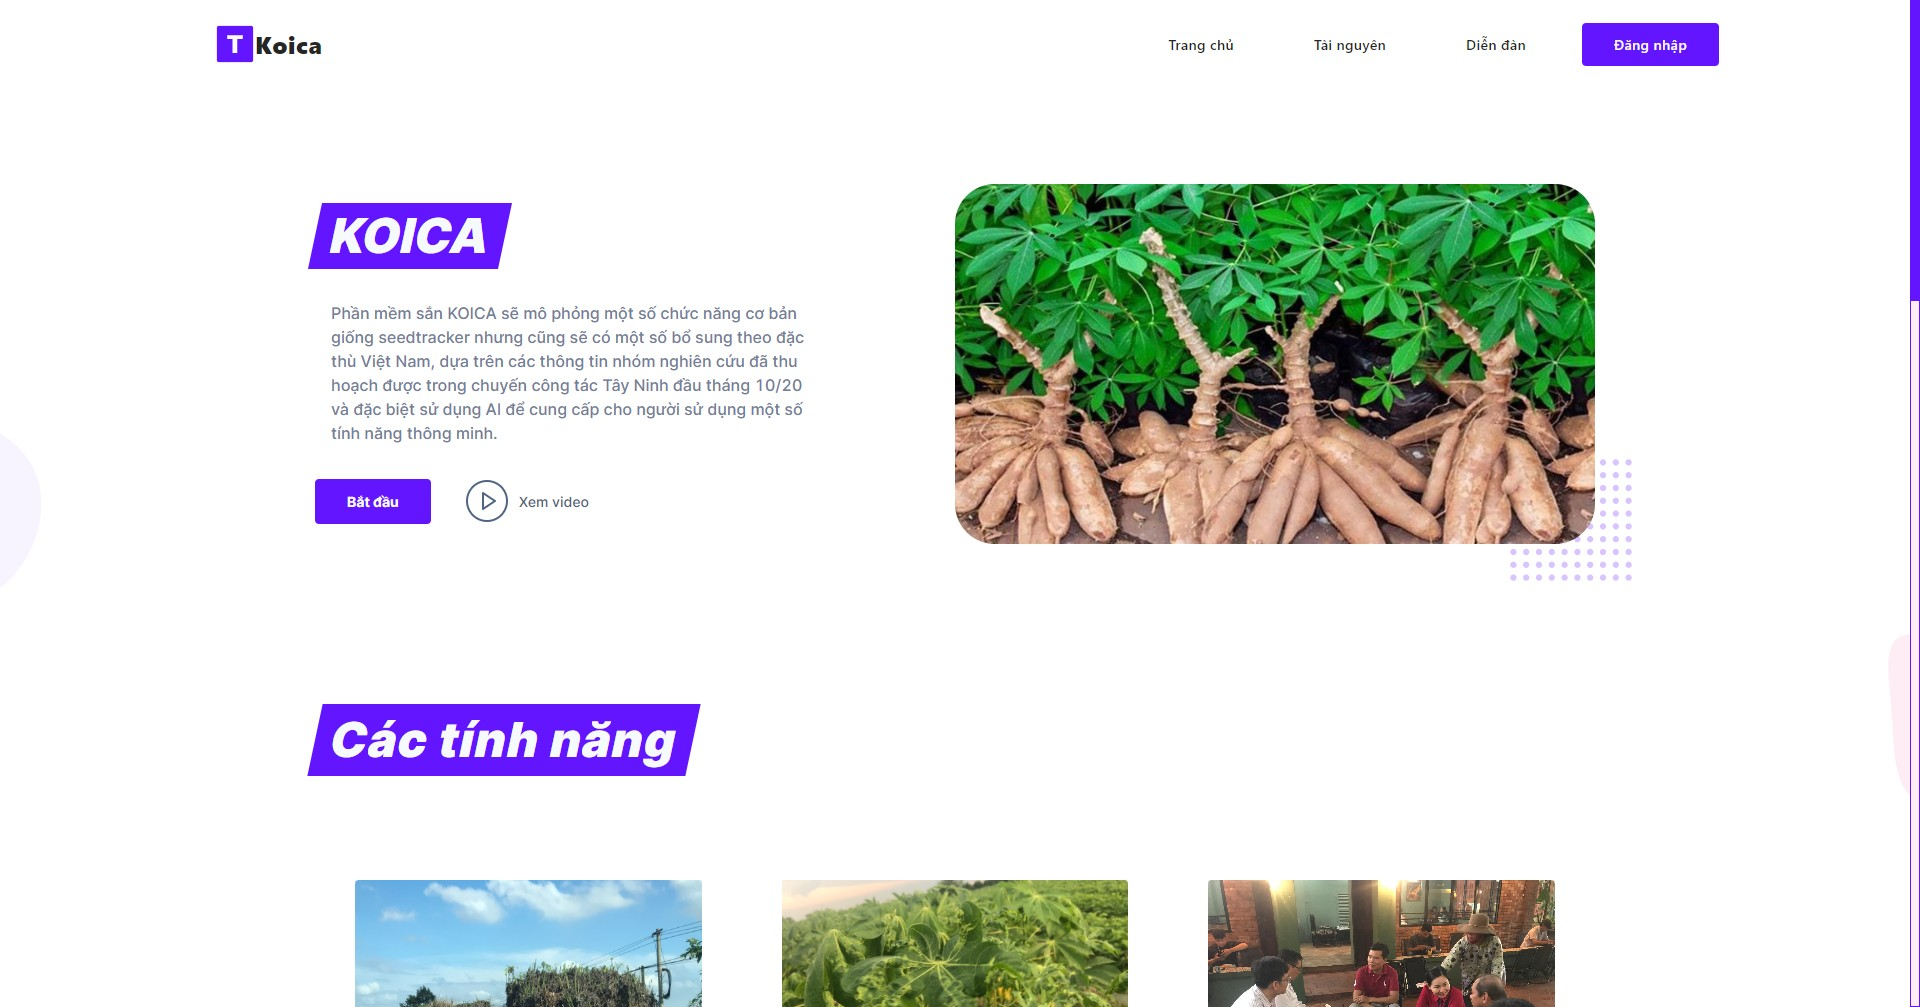
\includegraphics[height=0.34\textheight,keepaspectratio]{./img/test_hp1.jpeg}
        \caption{Kiểm thử giao diện trang chủ trên máy tính}
        \label{test:hp1}
    \end{figure}
    \begin{figure}[H]
    \centering
        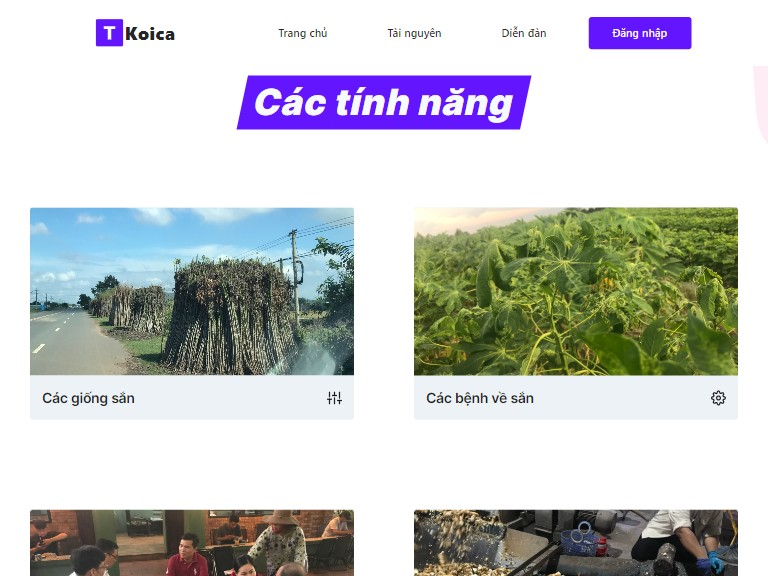
\includegraphics[height=0.45\textheight,keepaspectratio]{./img/test_hp2.jpeg}
        \caption{Kiểm thử giao diện trang chủ trên máy tính bảng}
        \label{test:hp2}
    \end{figure}
    \begin{figure}[H]
    \centering
        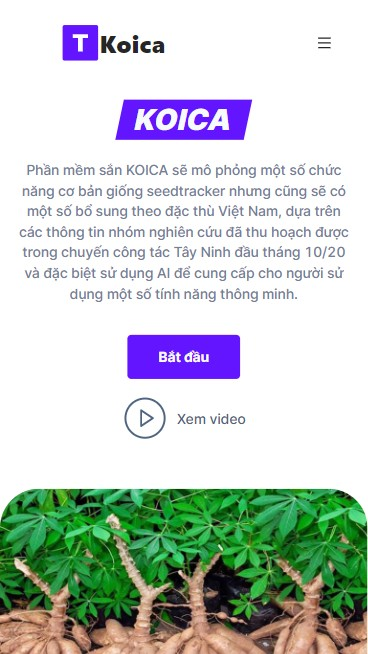
\includegraphics[height=0.4\textheight,keepaspectratio]{./img/test_hp3.jpeg}
        \caption{Kiểm thử giao diện trang chủ trên điện thoại}
        \label{test:hp3}
    \end{figure}
    \begin{figure}[H]
    \centering
        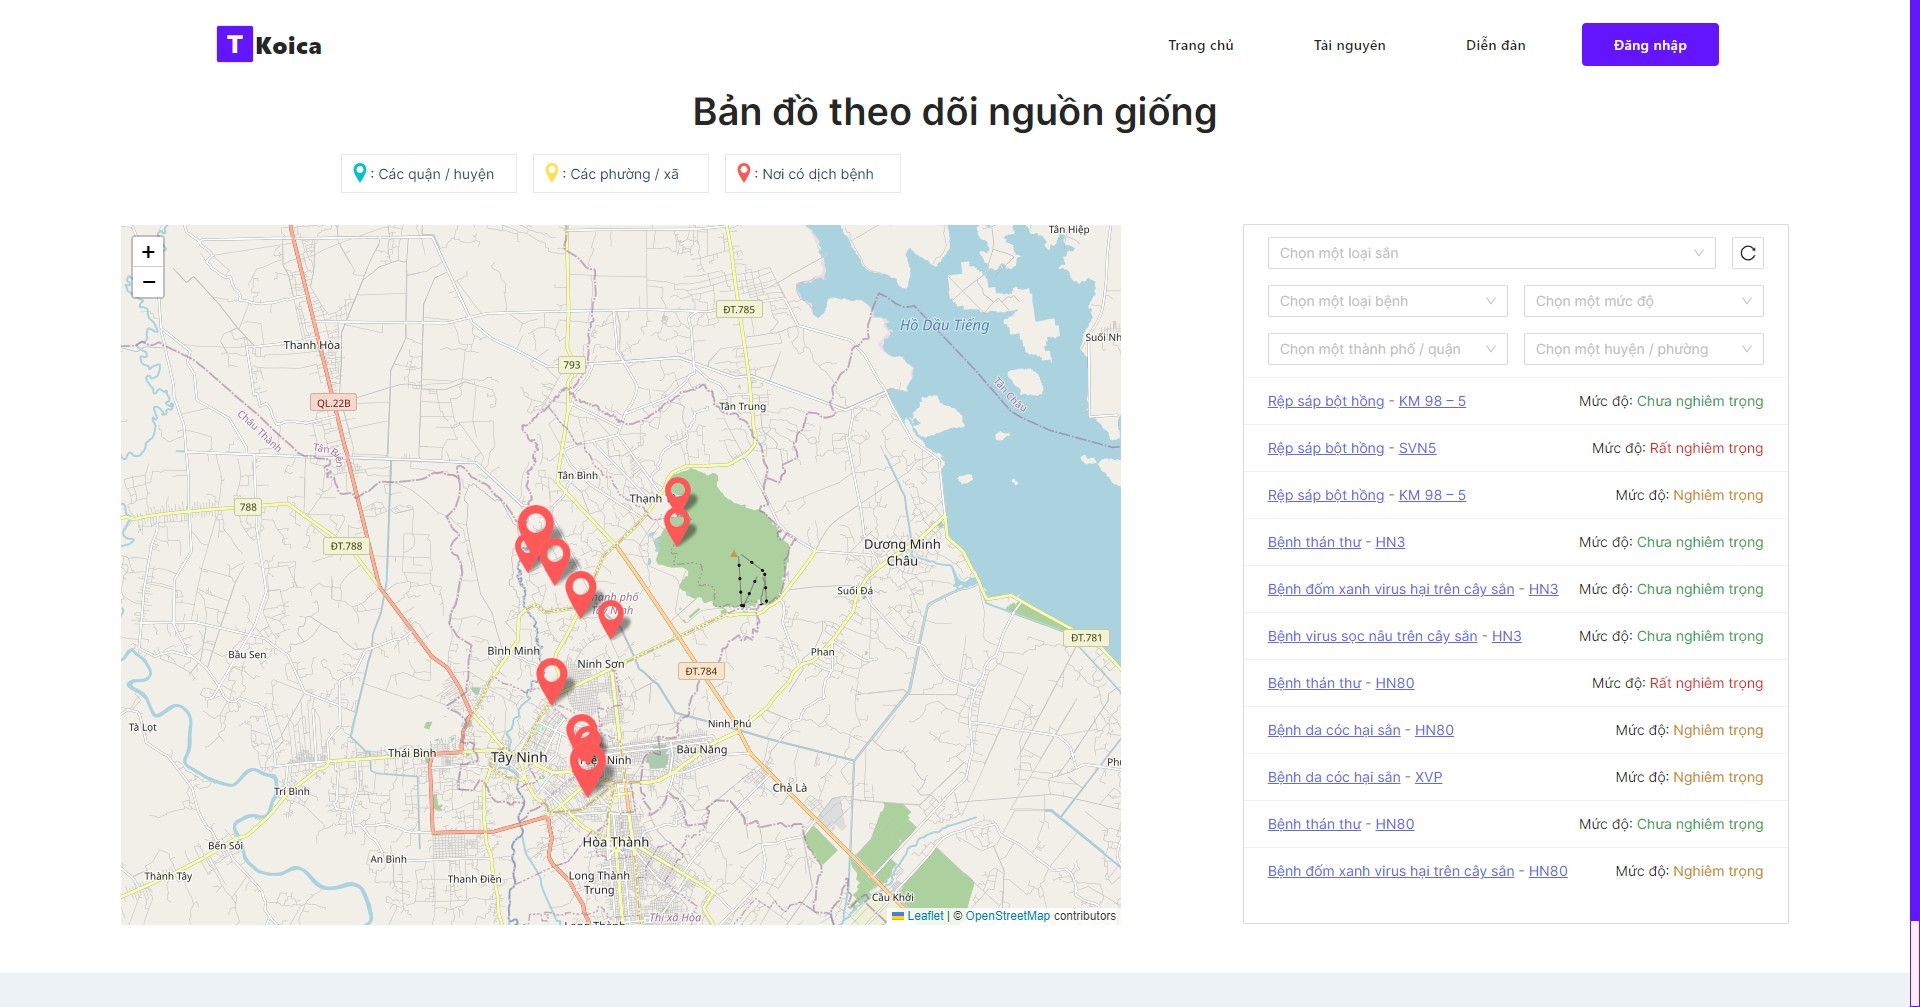
\includegraphics[height=0.34\textheight,keepaspectratio]{./img/test_map1.jpeg}
        \caption{Kiểm thử giao diện trang bản đồ sắn trên máy tính}
        \label{test:map1}
    \end{figure}
    \begin{figure}[H]
    \centering
        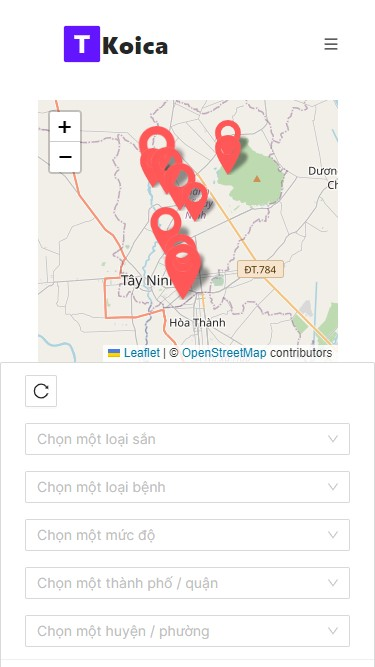
\includegraphics[height=0.5\textheight,keepaspectratio]{./img/test_map2.jpeg}
        \caption{Kiểm thử giao diện trang bản đồ sắn trên điện thoại}
        \label{test:map2}
    \end{figure}
    \begin{longtable}{| p{0.07\linewidth} | p{0.4\linewidth} | p{0.46\linewidth} |}
        \hline
        \textbf{STT} & \textbf{Kịch bản kiểm thử} & \textbf{Kết quả} \\ \hline
        \centerline{1} & - Giao diện trang chủ trên máy tính \newline - Hệ điều hành: Windows\newline - Trình duyệt: Google Chrome\newline - Kích thước máy: 1920px x 1080px & - Giao diện: Hình \ref{test:hp1}\newline - Nhận xét: Giao diện hiển thị giống như trong thiết kế, không bị vỡ bố cục trang. Các hiệu ứng chuyển động hiện ra khi kéo trang xuống dưới, thanh điều hướng hiển thị thêm hộp điều hướng khi di chuột qua.\\ \hline
        \centerline{2} & - Giao diện trang chủ trên máy tính bảng \newline - Hệ điều hành: Android\newline - Trình duyệt: Google Chrome\newline - Kích thước máy: 1024px x 768px & - Giao diện: Hình \ref{test:hp2}\newline - Nhận xét: Giao diện hiển thị tương đối giống thiết kế, không bị vỡ bố cục trang. Các ô nhỏ trong phần các tính năng được chia làm 2 cột thay vì 3 cột như xem trang chủ trên máy tính. Các mục khác hiển thị ổn, tuy nhiên vẫn còn bị lỗi thiếu khoảng cách so với viền trang.\\ \hline
        \centerline{3} & - Giao diện trang chủ trên điện thoại \newline - Hệ điều hành: Android \newline - Trình duyệt: Google Chrome\newline - Kích thước máy: 360px x 640px (Galaxy Note 3) & - Giao diện: Hình \ref{test:hp3}\newline - Nhận xét: Giao diện hiển thị giống như trong thiết kế, không bị vỡ bố cục trang. Thanh điều hướng trên cùng màn hình đã được chuyển thành một danh sách đường dẫn trang theo chiều dọc và ẩn đi, có thể đóng mở bằng cách bấm nút điều hướng ở góc trên bên phải màn hình. Phần các tính năng, bản đồ sắn, hỏi đáp và nhận xét phân chia theo chiều ngang trên máy tính đã được sắp xếp thành chiều dọc, phù hợp với chiều cao của điện thoại.\\ \hline
        \centerline{4} & - Giao diện trang bản đồ sắn trên máy tính \newline - Hệ điều hành: Ubuntu\newline - Trình duyệt: Microsoft Edge\newline - Kích thước máy: 1920px x 1080px & - Giao diện: Hình \ref{test:map1}\newline - Nhận xét: Giao diện hiển thị giống như trong thiết kế, không bị vỡ bố cục trang. Bên trái hiển thị bản đồ sắn có thể phóng to, thu nhỏ, có thể bấm vào các điểm đỏ để xem thông tin dịch bệnh đang diễn ra. Bên phải hiển thị bộ lọc tìm kiếm. Bản đồ hiển thị thông tin theo dữ liệu lọc được từ bộ lọc.\\ \hline
        \centerline{5} & - Giao diện trang bản đồ sắn trên điện thoại \newline - Hệ điều hành: macOS\newline - Trình duyệt: Google Chrome\newline - Kích thước máy: 375px x 667px (iPhone SE) & - Giao diện: Hình \ref{test:map2}\newline - Nhận xét: Giao diện hiển thị giống như trong thiết kế, không bị vỡ bố cục trang. Bản đồ và bộ lọc được sắp xếp theo chiều dọc, với bên trên là bản đồ, bên dưới là bộ lọc tìm kiếm. Vẫn giữ được khả năng tương tác với bản đồ như khi sử dụng máy tính.\\ \hline
        \caption{\label{test-ui}Kiểm thử tính linh hoạt của giao diện}
    \end{longtable}
    
    \item \textbf{Bảo mật hệ thống}: Quyền hạn của người dùng được phân chia theo 3 tác nhân chính đúng như tiêu chí đề ra. Những chức năng của quản trị viên sẽ chỉ có quản trị viên làm được, tương tự với người dùng. Với tác nhân khách sẽ có ít chức năng có thể thực hiện được nhất, hầu như chỉ là xem thông tin. Mật khẩu của các tài khoản sẽ được mã hóa lại trong cơ sở dữ liệu, tránh cho việc bị lấy cắp mật khẩu và làm lộ thông tin người dùng. Với các tác nhân có thêm các chức năng yêu cầu gửi kèm token còn khả dụng, thì khi token hết hiệu lực sẽ đăng xuất khỏi hệ thống, đảm bảo tính bảo mật đã đề ra.
    \item \textbf{Hiệu năng hoạt động}: Hệ thống đáp ứng được tối thiểu 100 người dùng cùng lúc và phản hồi dưới 1 giây mỗi yêu cầu. Với số lượng người dùng lớn hơn, phần mềm có thể bị hiện tượng đứng màn hình hiển thị, các thành phần trên giao diện bị sai lệch vị trí, cần phải khắc phục thêm.
    \item \textbf{Khả năng bảo trì}: Dữ liệu hệ thống có thể được xuất, nhập vào cơ sở dữ liệu bằng các thao tác đơn giản do quản trị viên thực hiện, đảm bảo khả năng phục hồi dữ liệu, tránh việc mất mát thông tin không đáng có. Các phiên bản cũng được lưu lại trên Github và luôn sẵn sàng cho việc quay trở lại phiên bản cũ bằng Docker compose.
\end{itemize}

\section{Nhận xét, đánh giá}
Như vậy, bằng việc áp dụng những nguyên lý thiết kế giao diện và hệ thống đã học, sản phẩm được phát triển có tính năng tương đối hoàn chỉnh và hỗ trợ đa nền tảng. Các yêu cầu chức năng và phi chức năng hầu hết đều được đáp ứng, song vẫn cần cải thiện nhiều chỗ về mặt giao diện, tối ưu hóa cơ sở dữ liệu,... để hoàn thiện hơn.

\end{document}